\chapter{LDA-Gaussian}
\label{A}
In this part of the appendix the results for all houses are shown for the LDA-Gaussian model. The number of time-slices is $n=48$ and the number of topics is $k=20$. The time dimension has a fine grain representation.

\paragraph{LDA-Gaussian}
Here the outcome of the LDA-Gaussian model is shown.

\begin{figure}[h!]
 \centering
 \begin{tabular}{c c}
  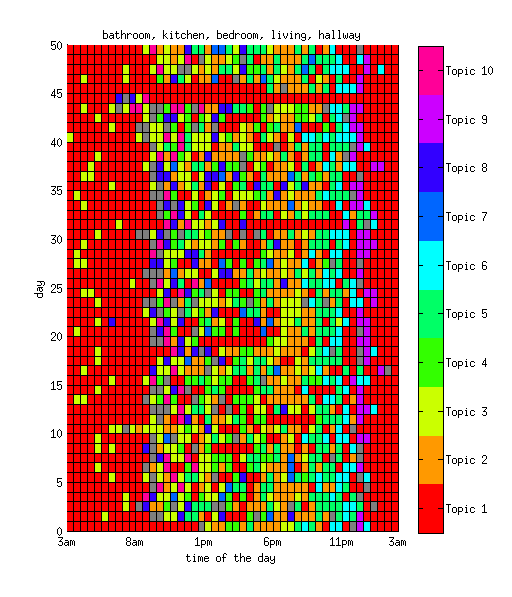
\includegraphics[width=0.45\textwidth]{Pictures/Gaus/fine/DayHN1TS48k20fine.png}
  &
  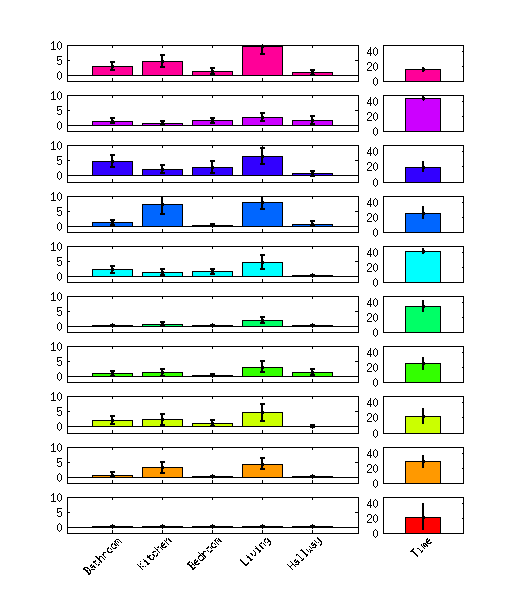
\includegraphics[width=0.45\textwidth]{Pictures/Gaus/fine/TopHN1TS48k20fine.png}\\
  a) & b)
 \end{tabular}
  \caption{House number 1, 20 topics, fine grain time, LDA-Gaussian}
\end{figure}

\begin{figure}[h!]
 \centering
 \begin{tabular}{c c}
  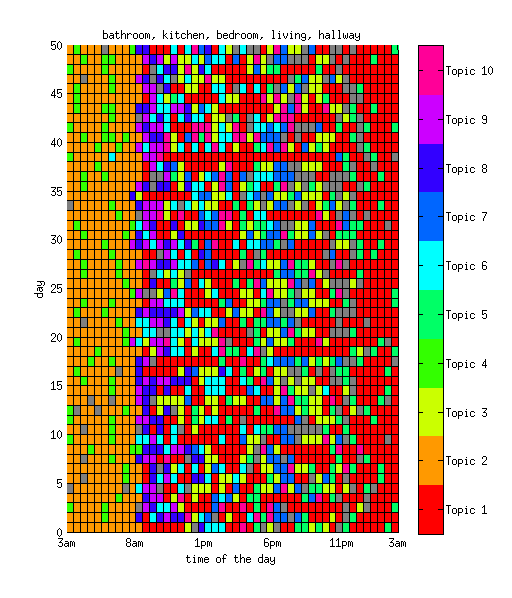
\includegraphics[width=0.45\textwidth]{Pictures/Gaus/fine/DayHN2TS48k20fine.png}
  &
  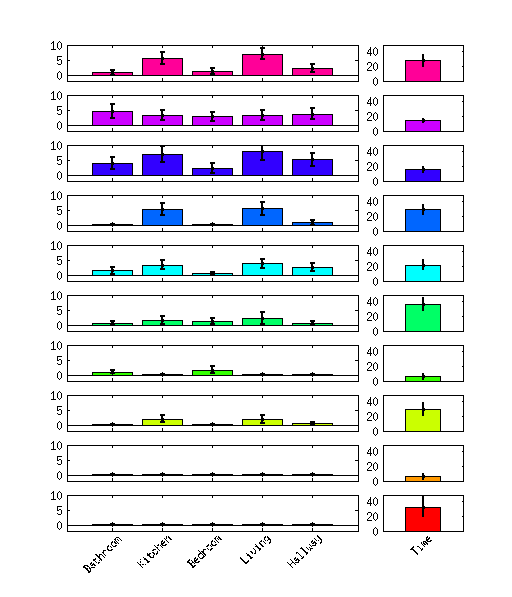
\includegraphics[width=0.45\textwidth]{Pictures/Gaus/fine/TopHN2TS48k20fine.png}\\
  a) & b)
 \end{tabular}
  \caption{House number 2, 20 topics, fine grain time, LDA-Gaussian}
\end{figure}

\begin{figure}[h!]
 \centering
 \begin{tabular}{c c}
  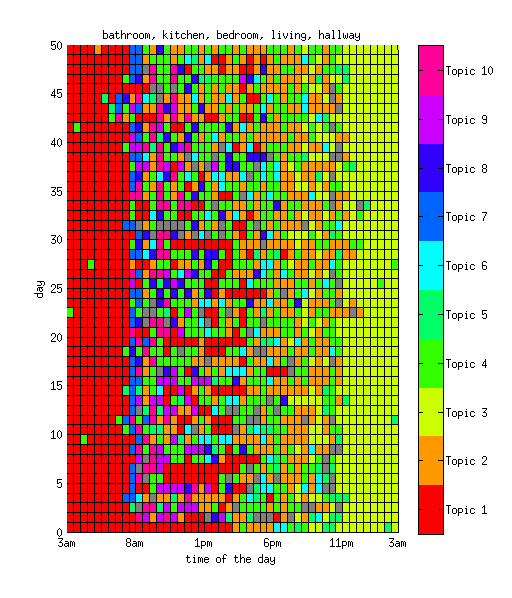
\includegraphics[width=0.45\textwidth]{Pictures/Gaus/fine/DayHN3TS48k20fine.png}
  &
  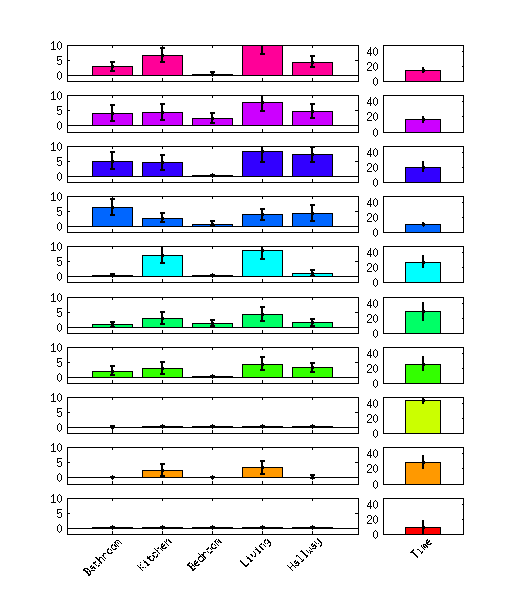
\includegraphics[width=0.45\textwidth]{Pictures/Gaus/fine/TopHN3TS48k20fine.png}\\
  a) & b)
 \end{tabular}
  \caption{House number 3, 20 topics, fine grain time, LDA-Gaussian}
\end{figure}

\begin{figure}[h!]
 \centering
 \begin{tabular}{c c}
  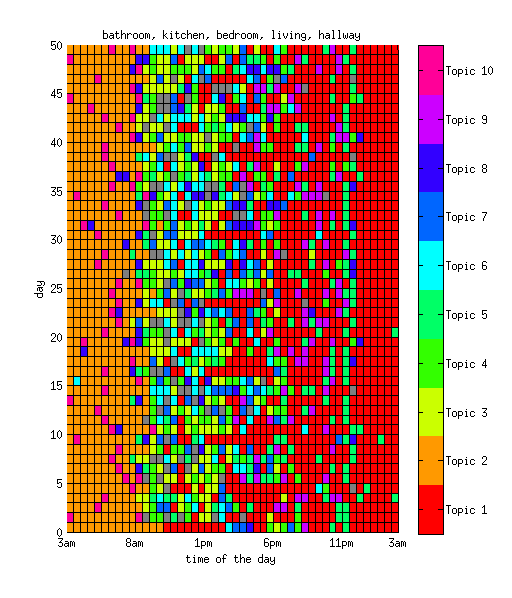
\includegraphics[width=0.45\textwidth]{Pictures/Gaus/fine/DayHN4TS48k20fine.png}
  &
  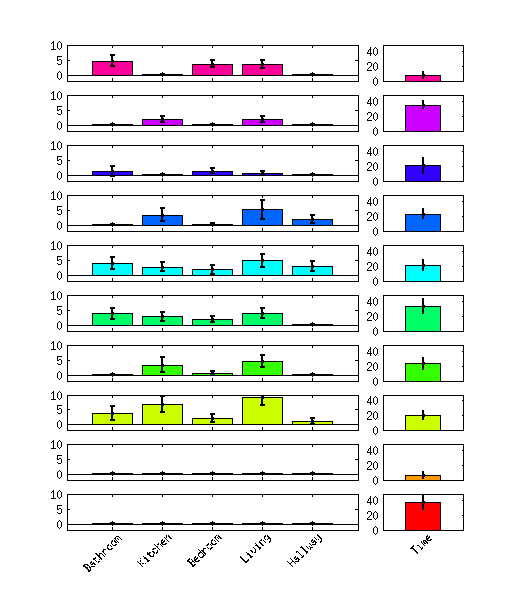
\includegraphics[width=0.45\textwidth]{Pictures/Gaus/fine/TopHN4TS48k20fine.png}\\
  a) & b)
 \end{tabular}
  \caption{House number 4, 20 topics, fine grain time, LDA-Gaussian}
\end{figure}

\begin{figure}[h!]
 \centering
 \begin{tabular}{c c}
  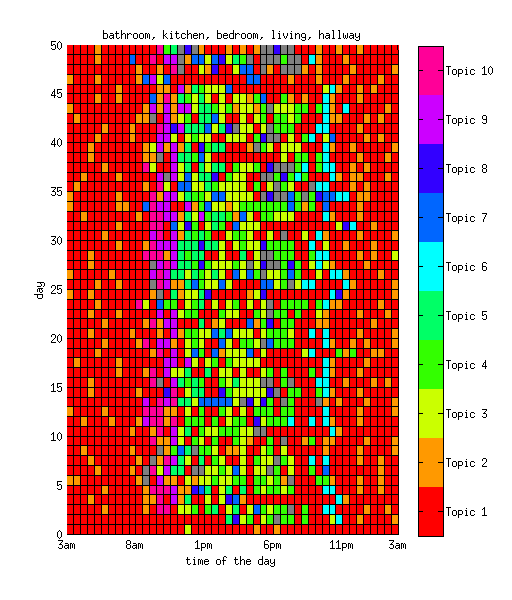
\includegraphics[width=0.45\textwidth]{Pictures/Gaus/fine/DayHN5TS48k20fine.png}
  &
  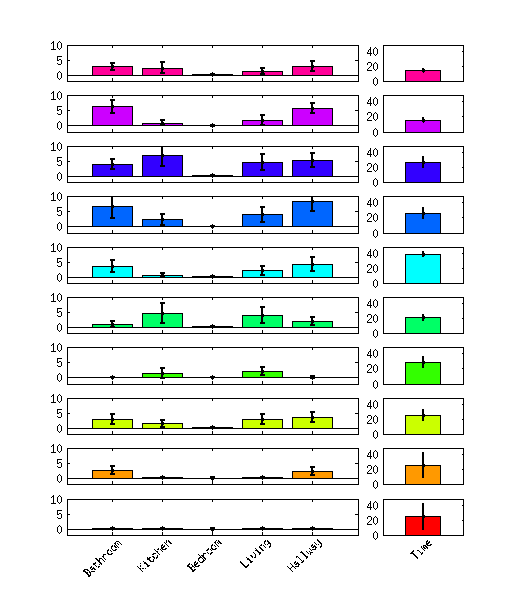
\includegraphics[width=0.45\textwidth]{Pictures/Gaus/fine/TopHN5TS48k20fine.png}\\
  a) & b)
 \end{tabular}
  \caption{House number 5, 20 topics, fine grain time, LDA-Gaussian}
\end{figure}

\chapter{LDA-Poisson}
\label{B}
Here the results for all houses are shown for the LDA-Poisson model. The number of time-slices is $n=48$ and the number of topics is $k=20$. The time dimension has a fine grain representation.


\begin{figure}[h!]
 \centering
 \begin{tabular}{c c}
  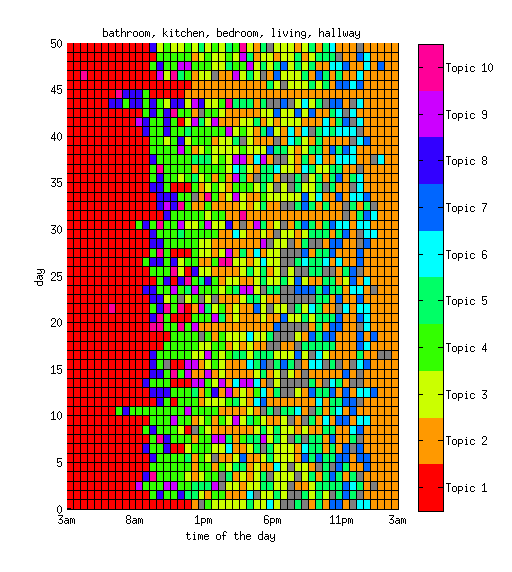
\includegraphics[width=0.45\textwidth]{Pictures/Pois/fine/DayHN1TS48k20fine.png}
  &
  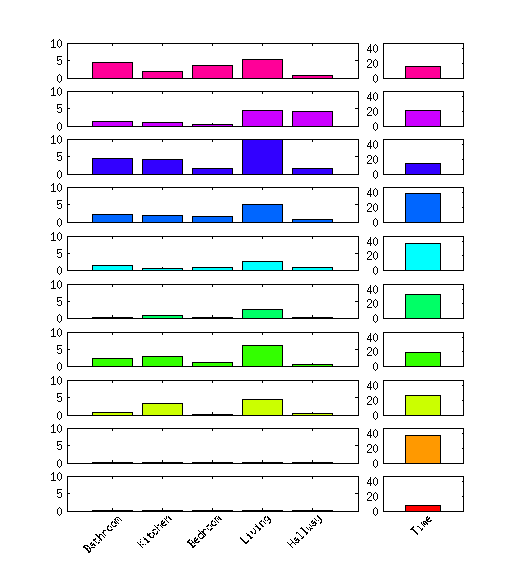
\includegraphics[width=0.45\textwidth]{Pictures/Pois/fine/TopHN1TS48k20fine.png}\\
  a) & b)
 \end{tabular}
  \caption{House number 1, 20 topics, fine grain time, LDA-Poisson}
\end{figure}

\begin{figure}[h!]
 \centering
 \begin{tabular}{c c}
  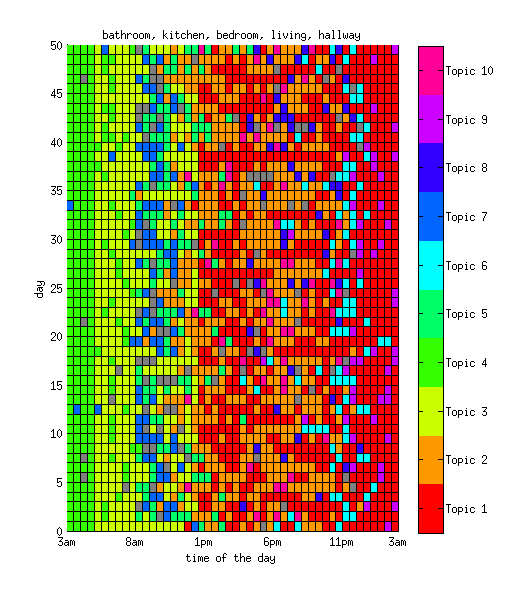
\includegraphics[width=0.45\textwidth]{Pictures/Pois/fine/DayHN2TS48k20fine.png}
  &
  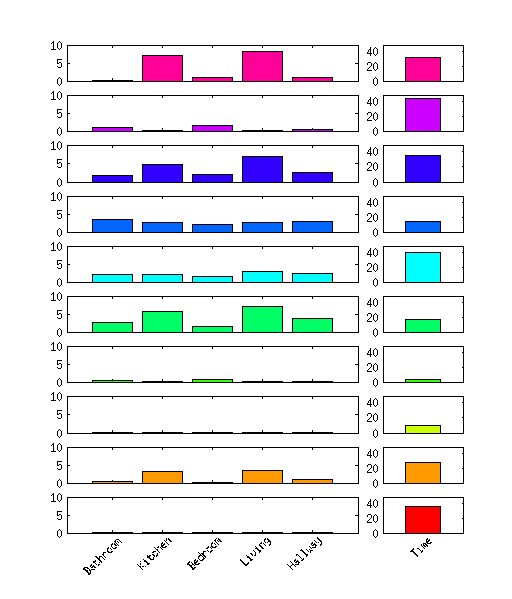
\includegraphics[width=0.45\textwidth]{Pictures/Pois/fine/TopHN2TS48k20fine.png}\\
  a) & b)
 \end{tabular}
  \caption{House number 2, 20 topics, fine grain time, LDA-Poisson}
\end{figure}

\begin{figure}[h!]
 \centering
 \begin{tabular}{c c}
  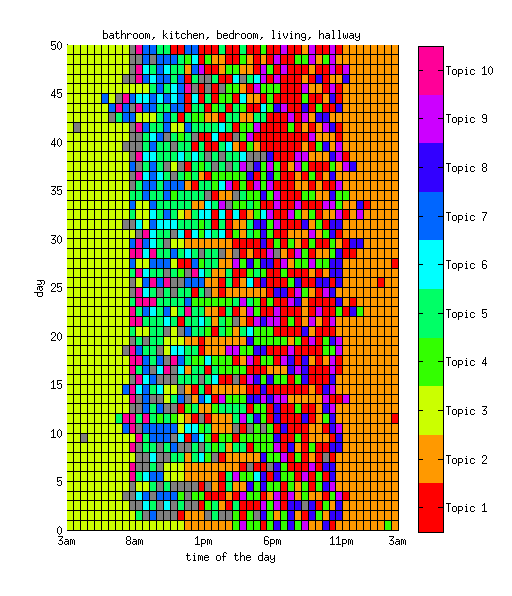
\includegraphics[width=0.45\textwidth]{Pictures/Pois/fine/DayHN3TS48k20fine.png}
  &
  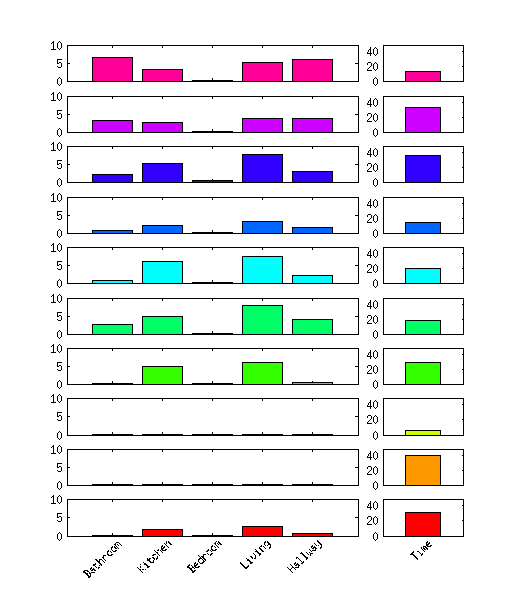
\includegraphics[width=0.45\textwidth]{Pictures/Pois/fine/TopHN3TS48k20fine.png}\\
  a) & b)
 \end{tabular}
  \caption{House number 3, 20 topics, fine grain time, LDA-Poisson}
\end{figure}

\begin{figure}[h!]
 \centering
 \begin{tabular}{c c}
  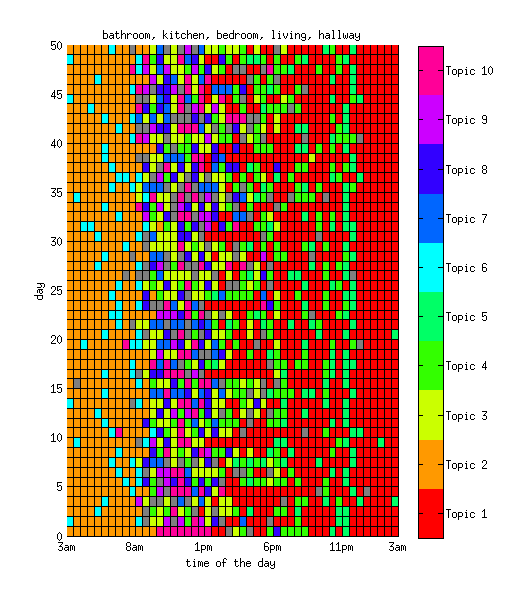
\includegraphics[width=0.45\textwidth]{Pictures/Pois/fine/DayHN4TS48k20fine.png}
  &
  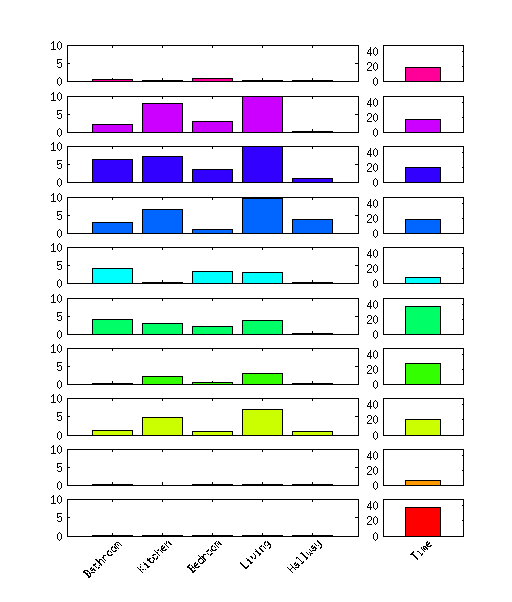
\includegraphics[width=0.45\textwidth]{Pictures/Pois/fine/TopHN4TS48k20fine.png}\\
  a) & b)
 \end{tabular}
  \caption{House number 4, 20 topics, fine grain time, LDA-Poisson}
\end{figure}

\begin{figure}[h!]
 \centering
 \begin{tabular}{c c}
  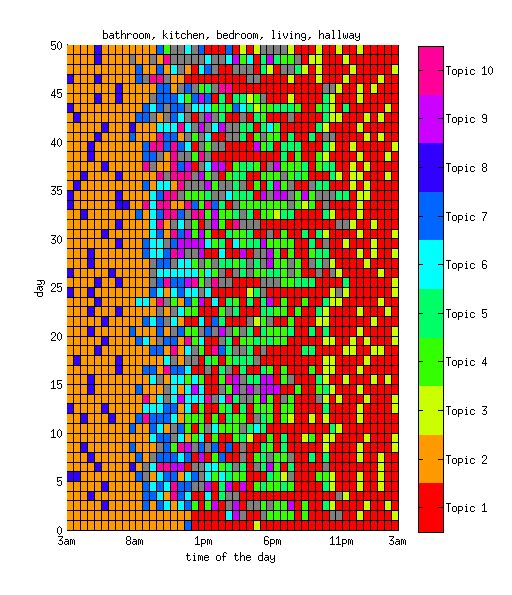
\includegraphics[width=0.45\textwidth]{Pictures/Pois/fine/DayHN5TS48k20fine.png}
  &
  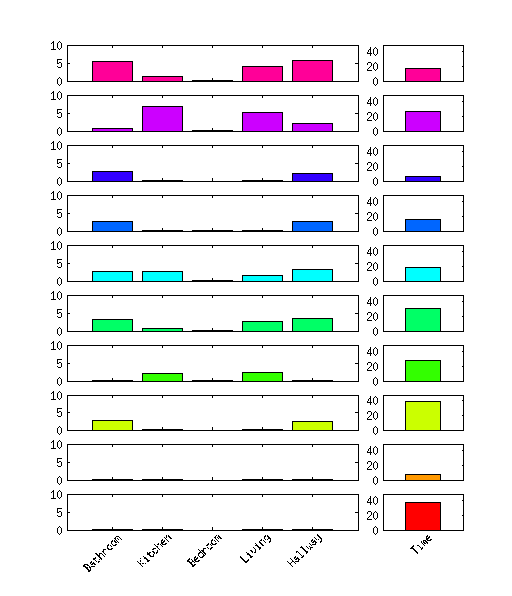
\includegraphics[width=0.45\textwidth]{Pictures/Pois/fine/TopHN5TS48k20fine.png}\\
  a) & b)
 \end{tabular}
  \caption{House number 5, 20 topics, fine grain time, LDA-Poisson}
\end{figure}